%%%%%%%%%%%%%%%%%%%%%%%%%%%%%%%%%%%%%%%%%%%%%%%%%%%%%%%%%%%%%%%%%%%%%%%%%%%%%%%%
% extendible_hashing.tex
% An example demonstrating how to show extendible hashing in LaTeX with TikZ
% https://github.com/mhyee/latex-examples/
%%%%%%%%%%%%%%%%%%%%%%%%%%%%%%%%%%%%%%%%%%%%%%%%%%%%%%%%%%%%%%%%%%%%%%%%%%%%%%%%


% LaTeX Preamble
% Load packages and set options as needed
%%%%%%%%%%%%%%%%%%%%%%%%%%%%%%%%%%%%%%%%%%%%%%%%%%%%%%%%%%%%%%%%%%%%%%%%%%%%%%%%

% Set the document class to "article"
% Pass it "12pt" and "letterpaper" options
\documentclass[12pt,letterpaper]{article}

% We don't need the special font encodings, but still
% good practice to include these. See:
%
% http://tex.stackexchange.com/questions/664/why-should-i-use-usepackaget1fontenc
% http://dsanta.users.ch/resources/type1.html
\usepackage[T1]{fontenc}
\usepackage{ae,aecompl}
% http://tex.stackexchange.com/a/44699
% http://tex.stackexchange.com/a/44701
\usepackage[utf8]{inputenc}

% Use Latin Modern, an improved version of the Computer Modern font
\usepackage{lmodern}

% TikZ is what lets us draw graphics
\usepackage{tikz}
% We want to be able to draw shapes (rectangles) with multiple parts in them
\usetikzlibrary{shapes.multipart}

% Disable page numbering
\pagestyle{empty}

% Define our own macros, for convenience
%%%%%%%%%%%%%%%%%%%%%%%%%%%%%%%%%%%%%%%%%%%%%%%%%%%%%%%%%%%%%%%%%%%%%%%%%%%%%%%%

% \ensuremath{ARG} is used to enable mathematics mode in a macro
% ARG will always be rendered in math mode,
% regardless of which mode the macro is called in
%
% http://www.giss.nasa.gov/tools/latex/ensuremath.html

% \block{KB_VAL}{NUM_PARTS}{ID}{CONTENTS} becomes
% node[label=above:{\ensuremath{k_B=KB_VAL}},rectangle split, rectangle split parts=NUM_PARTS](ID) {CONTENTS}
\newcommand{\block}[4]{node[label=above:{\ensuremath{k_B=#1}},rectangle split, rectangle split parts=#2](#3) {#4}}

% Begin the actual typesetting, by starting the "document" environment
%%%%%%%%%%%%%%%%%%%%%%%%%%%%%%%%%%%%%%%%%%%%%%%%%%%%%%%%%%%%%%%%%%%%%%%%%%%%%%%%
\begin{document}

% This diagram is essentially a sideways tree, with height 1.
% The structure is something like this:
%
%      h(424)=0
% 0 /
% 1 /  h(109)=5
% 2 -  h(132)=4
% 3    h(244)=4
%   \
%      h(775)=7
%
% Note that 0 and 1 point to h(424)=0.

  \begin{center}
    % Show the hashing function
    \[ h(k) = k \bmod{8} \]

    % Now we draw the picture, with the following options:
    % - grow the tree from left to right (instead of top to bottom)
    % - set up the distance/spacing for the first child level
    % - don't draw the default edges
    % - define the "pointer" and "dpointer" edges, which differ in length
    % - set up styles for ever label and every node
    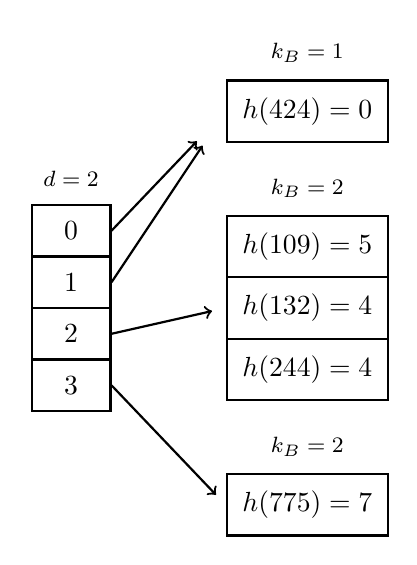
\begin{tikzpicture}[
      grow=right,
      level 1/.style={sibling distance=2.5cm,level distance=3cm},
      edge from parent/.style={draw=none},
      pointer/.style={thick, shorten >=5pt, ->,draw=black},
      dpointer/.style={thick, shorten >=15pt, ->,draw=black},
      every label/.style={font=\footnotesize,draw=none},
      every node/.style={rectangle,thick,draw=black, text ragged, inner sep=2mm,minimum width=10mm}
      ]

      % Draw the root node, give it the id "directory"
      % There is a label above the node, and the node is a rectangle split into 4 parts, each with a label (eg one) and contents (eg 0).
      \node[label=above:{$d=2$},rectangle split, rectangle split parts=4] (directory) {
        \nodepart{one} 0
        \nodepart{two} 1
        \nodepart{three} 2
        \nodepart{four} 3
      }
      % The node has three children
      % Note that the first child is at the bottom, while the last is at the top
      % This corresponds to a regular tree (first=left) rotated 90 degrees counterclockwise

        % This is semantically the last child, so it goes on the bottom
        % But because of the ordering, we have to list it first

        % We're using the macro we defined previously:
        % k_B = 2, one part, the id is c, and the contents are "h(775)=7"

        % For the second child, note how \nodepart acts as a separator
        % Warning: There must not be any blank lines between these children, otherwise we get a child of a child instead of siblings.
        child {
          \block{2}{1}{c}{ $h(775)=7$ }
        }
        child {
          \block{2}{3}{b}{ $h(109)=5$ \nodepart{second} $h(132)=4$ \nodepart{third} $h(244)=4$ }
        }
        child {
          \block{1}{1}{a}{ $h(424)=0$ }
        };

      % Now we set up the pointers

      % directory.one refers to the rectangular part "one" within the "directory" node. We draw an edge from its east (right) side to node a's west (left).
      % Use the edge style dpointer, because we have a double pointer to node a. dpointer is shorter than pointer, so it'll look nicer.
      \path(directory.one east) edge [dpointer] (a.west);
      \path(directory.two east) edge [dpointer] (a.west);
      \path(directory.three east) edge [pointer] (b.west);
      \path(directory.four east) edge [pointer] (c.west);
    \end{tikzpicture}
  \end{center}

\end{document}
